\iffalse
This file is protected by Copyright. Please refer to the COPYRIGHT file
distributed with this source distribution.

This file is part of OpenCPI <http://www.opencpi.org>

OpenCPI is free software: you can redistribute it and/or modify it under the
terms of the GNU Lesser General Public License as published by the Free Software
Foundation, either version 3 of the License, or (at your option) any later
version.

OpenCPI is distributed in the hope that it will be useful, but WITHOUT ANY
WARRANTY; without even the implied warranty of MERCHANTABILITY or FITNESS FOR A
PARTICULAR PURPOSE. See the GNU Lesser General Public License for more details.

You should have received a copy of the GNU Lesser General Public License along
with this program. If not, see <http://www.gnu.org/licenses/>.
\fi
%----------------------------------------------------------------------------------------
% Update the docTitle and docVersion per document
%----------------------------------------------------------------------------------------
\def\docTitle{Configure Environment for ModelSim}
\def\docVersion{1.2}
%----------------------------------------------------------------------------------------
\documentclass{article}
\iffalse
This file is protected by Copyright. Please refer to the COPYRIGHT file
distributed with this source distribution.

This file is part of OpenCPI <http://www.opencpi.org>

OpenCPI is free software: you can redistribute it and/or modify it under the
terms of the GNU Lesser General Public License as published by the Free Software
Foundation, either version 3 of the License, or (at your option) any later
version.

OpenCPI is distributed in the hope that it will be useful, but WITHOUT ANY
WARRANTY; without even the implied warranty of MERCHANTABILITY or FITNESS FOR A
PARTICULAR PURPOSE. See the GNU Lesser General Public License for more details.

You should have received a copy of the GNU Lesser General Public License along
with this program. If not, see <http://www.gnu.org/licenses/>.
\fi
\author{} % Force author to be blank
%----------------------------------------------------------------------------------------
% Paper size, orientation and margins
%----------------------------------------------------------------------------------------
\usepackage{geometry}
\geometry{
        letterpaper, % paper type
        portrait,    % text direction
        left=.75in,  % left margin
        top=.75in,   % top margin
        right=.75in, % right margin
        bottom=.75in % bottom margin
 }
%----------------------------------------------------------------------------------------
% Header/Footer
%----------------------------------------------------------------------------------------
\usepackage{fancyhdr} \pagestyle{fancy} % required for fancy headers
\renewcommand{\headrulewidth}{0.5pt}
\renewcommand{\footrulewidth}{0.5pt}
\rhead{\small{ANGRYVIPER Team}}
% \rfoot{\thepage}
%----------------------------------------------------------------------------------------
% Appendix packages
%----------------------------------------------------------------------------------------
\usepackage[toc,page]{appendix}
%----------------------------------------------------------------------------------------
% Defined Commands & Renamed Commands
%----------------------------------------------------------------------------------------
\renewcommand{\contentsname}{Table of Contents}
\renewcommand{\listfigurename}{List of Figures}
\renewcommand{\listtablename}{List of Tables}
%----------------------------------------------------------------------------------------
% Various packages
%----------------------------------------------------------------------------------------
\usepackage[usenames,dvipsnames]{xcolor} % for color names see https://en.wikibooks.org/wiki/LaTeX/Colors
\usepackage{hyperref}  % for linking urls and lists
\usepackage{graphicx}  % for including pictures by file
\usepackage{listings}  % for coding language styles
\usepackage{rotating}  % for sideways table
\usepackage{pifont}    % for sideways table
\usepackage{pdflscape} % for landscape view
\usepackage{subfig}
\usepackage{xstring}
\uchyph=0 % Never hyphenate acronyms like RCC (I think this overrides ANGRYVIPER above)
\renewcommand\_{\textunderscore\allowbreak} % Allow words to break/newline on underscores
%----------------------------------------------------------------------------------------
% Table packages
%----------------------------------------------------------------------------------------
\usepackage{longtable} % for long possibly multi-page tables
\usepackage{tabularx} % c=center,l=left,r=right,X=fill
% These define tabularx columns "C" and "R" to match "X" but center/right aligned
\newcolumntype{C}{>{\centering\arraybackslash}X}
\newcolumntype{R}{>{\raggedleft\arraybackslash}X}
\usepackage{float}
\floatstyle{plaintop}
\usepackage[tableposition=top]{caption}
\newcolumntype{P}[1]{>{\centering\arraybackslash}p{#1}}
\newcolumntype{M}[1]{>{\centering\arraybackslash}m{#1}}
%----------------------------------------------------------------------------------------
% Block Diagram / FSM Drawings
%----------------------------------------------------------------------------------------
\usepackage{tikz}
\usetikzlibrary{shapes,arrows,fit,positioning}
\usetikzlibrary{automata} % used for the fsm
%----------------------------------------------------------------------------------------
% Colors Used
%----------------------------------------------------------------------------------------
\usepackage{colortbl}
\definecolor{blue}{rgb}{.7,.8,.9}
\definecolor{ceruleanblue}{rgb}{0.16, 0.32, 0.75}
\definecolor{drkgreen}{rgb}{0,0.6,0}
\definecolor{deepmagenta}{rgb}{0.8, 0.0, 0.8}
\definecolor{cyan}{rgb}{0.0,0.6,0.6}
\definecolor{maroon}{rgb}{0.5,0,0}
%----------------------------------------------------------------------------------------
% VHDL Coding Language Style
% modified from: http://latex-community.org/forum/viewtopic.php?f=44&t=22076
%----------------------------------------------------------------------------------------
\lstdefinelanguage{VHDL}
{
        basicstyle=\ttfamily\footnotesize,
        columns=fullflexible,keepspaces,      % https://tex.stackexchange.com/a/46695/87531
        keywordstyle=\color{ceruleanblue},
        commentstyle=\color{drkgreen},
        morekeywords={
    library,use,all,entity,is,port,in,out,end,architecture,of,
    begin,and, signal, when, if, else, process, end,
        },
        morecomment=[l]--
}
%----------------------------------------------------------------------------------------
% XML Coding Language Style
% modified from: http://tex.stackexchange.com/questions/10255/xml-syntax-highlighting
%----------------------------------------------------------------------------------------
\lstdefinelanguage{XML}
{
        basicstyle=\ttfamily\footnotesize,
        columns=fullflexible,keepspaces,
        morestring=[s]{"}{"},
        morecomment=[s]{!--}{--},
        commentstyle=\color{drkgreen},
        moredelim=[s][\color{black}]{>}{<},
        moredelim=[s][\color{cyan}]{\ }{=},
        stringstyle=\color{maroon},
        identifierstyle=\color{ceruleanblue}
}
%----------------------------------------------------------------------------------------
% DIFF Coding Language Style
% modified from http://tex.stackexchange.com/questions/50176/highlighting-a-diff-file
%----------------------------------------------------------------------------------------
\lstdefinelanguage{diff}
{
        basicstyle=\ttfamily\footnotesize,
        columns=fullflexible,keepspaces,
        breaklines=true,                                % wrap text
        morecomment=[f][\color{ceruleanblue}]{@@},      % group identifier
        morecomment=[f][\color{red}]-,                  % deleted lines
        morecomment=[f][\color{drkgreen}]+,             % added lines
        morecomment=[f][\color{deepmagenta}]{---},      % Diff header lines (must appear after +,-)
        morecomment=[f][\color{deepmagenta}]{+++},
}
%----------------------------------------------------------------------------------------
% Python Coding Language Style
% modified from
%----------------------------------------------------------------------------------------
\lstdefinelanguage{python}
{
        basicstyle=\ttfamily\footnotesize,
        columns=fullflexible,keepspaces,
        keywordstyle=\color{ceruleanblue},
        commentstyle=\color{drkgreen},
        stringstyle=\color{orange},
        morekeywords={
    print, if, sys, len, from, import, as, open,close, def, main, for, else, write, read, range,
        },
        comment=[l]{\#}
}
%----------------------------------------------------------------------------------------
% Fontsize Notes in order from smallest to largest
%----------------------------------------------------------------------------------------
%    \tiny
%    \scriptsize
%    \footnotesize
%    \small
%    \normalsize
%    \large
%    \Large
%    \LARGE
%    \huge
%    \Huge

\date{Version \docVersion} % Force date to be blank and override date with version
\title{\docTitle}
\lhead{\docTitle}
%----------------------------------------------------------------------------------------
\graphicspath{ {figures/} }

\begin{document}
\maketitle
\thispagestyle{fancy}
\newpage

	\begin{center}
	\textit{\textbf{Revision History}}
		\begin{table}[H]
		\label{table:revisions} % Add "[H]" to force placement of table
			\begin{tabularx}{\textwidth}{|c|X|l|}
			\hline
			\rowcolor{blue}
			\textbf{Revision} & \textbf{Description of Change} & \textbf{Date} \\
		    \hline
		    v1.0 & Initial Release & 2/2016 \\
		    \hline
			v1.1 & Updated for OpenCPI 1.1 & 3/2017 \\
			\hline
			v1.2 & Updated for OpenCPI 1.2 & 8/2017 \\
			\hline
			\end{tabularx}
		\end{table}
	\end{center}

\newpage

\tableofcontents

\newpage
\iffalse
% Removed this unneeded section. The table is all broken - link is a Xilinx UG? Was that supposed to be a different link? We don't have a Technical Summary document, do we? etc...

\section{References}

	This document assumes a basic understanding of the Linux command line (or ``shell'') environment. It requires a working knowledge of OpenCPI and FPGA vendor tools. The reference(s) in Table \ref{table:references} can be used as an overview of OpenCPI and may prove useful.

	\begin{center}
		\begin{table}[H]
		\caption {References}
		\label{table:references}
			\begin{tabularx}{\textwidth}{|c|c|X|}
			\hline
			\rowcolor{blue}
			\textbf{Title} & \textbf{Published By} & \textbf{Link} \\
			\hline
			Technical Summary & OpenCPI & UG628 Command Line Tools User Guide \\
		    \hline
			 & & \\
			\hline
			\end{tabularx}
		\end{table}
	\end{center}

\newpage
\fi
\section{Overview}

	This document describes how to compile Xilinx simulation libraries of a device(s) for a particular 3rd party simulator, such as ModelSim.

	\begin{enumerate}
	 	\item Compile Xilinx libraries for ModelSim
		\item Modify \texttt{modelsim.ini} to include path of compiled Xilinx libraries
	\end{enumerate}

\section{Compile Xilinx/Zynq simulation libraries for ModelSim}
\subsection{Compile Vivado's simulation libraries}
	This section provides the steps necessary to compile Xilinx Vivado's simulation libraries of the Zynq device, for ModelSim. If using Modelsim 10.4c, note that Vivado 2017.1 does not support compilation of simulation libraries for ModelSim versions earlier than 10.5c. Therefore, if using a ModelSim 10.4c, you will need to use an earlier version of Vivado (\textit{e.g} 2015.4) to compile the simulation libraries. For this example, we use Vivado 2017.1 with Modelsim DE 10.6a.

\begin{flushleft}
	\begin{enumerate}
		\item Open a terminal window and switch the user to root:
			\subitem \code{> sudo su -}
		\item Configure the terminal for Xilinx Vivado by sourcing the setup script (for bash):
			\subitem \code{> source /opt/Xilinx/Vivado/<version>/settings64.sh}
		\item Launch Vivado:
			\subitem \code{> vivado}
		\item Select Tools $\rightarrow$ Compile Simulation Libraries...
		\item Select the following:
			\subitem Simulator: Modelsim Simulator
			\subitem Language: VHDL
			\subitem Library: All
			\subitem Family: Zynq-7000
			\subitem Compiled library location: \path{/opt/Xilinx/Vivado/<version>/vhdl/modelsim/<version>/lin64}
			\subitem Simulator executable path: \path{/opt/Modelsim/modelsim_dlx/linuxpe}
			\subitem Compile 32-bit libraries: Yes

		\begin{figure}[H]
	\centering\captionsetup{type=figure}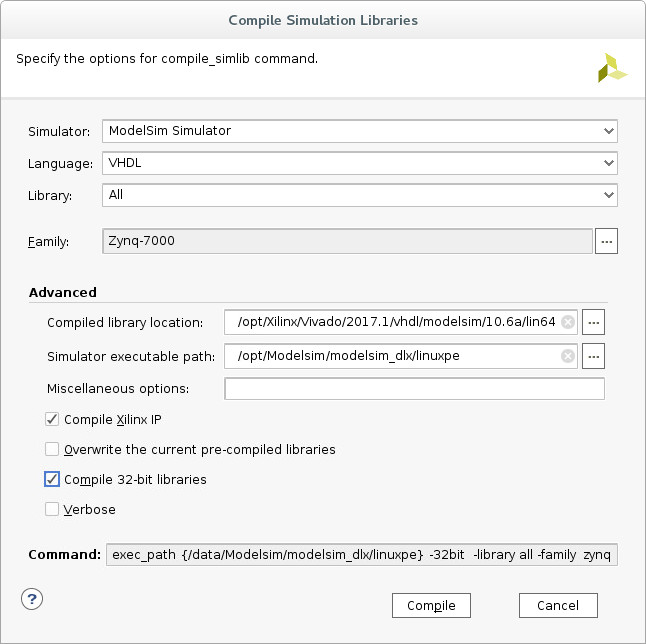
\includegraphics[scale=0.5]{xilinx_vivado_complibrary}
		\captionof{figure}{Vivado 2017.1 Compile Simulation Libraries}
	\end{figure}
		\item Click ``Compile''
		\item Note that 2017.1 Vivado will result in errors for Modelsim versions earlier than 10.5c. Here, we show the results for Vivado 2017.1 with Modelsim DE 10.6a, and Vivado 2015.4 with Modelsim DE 10.4c.
	\begin{figure}[H]
	\centering\captionsetup{type=figure}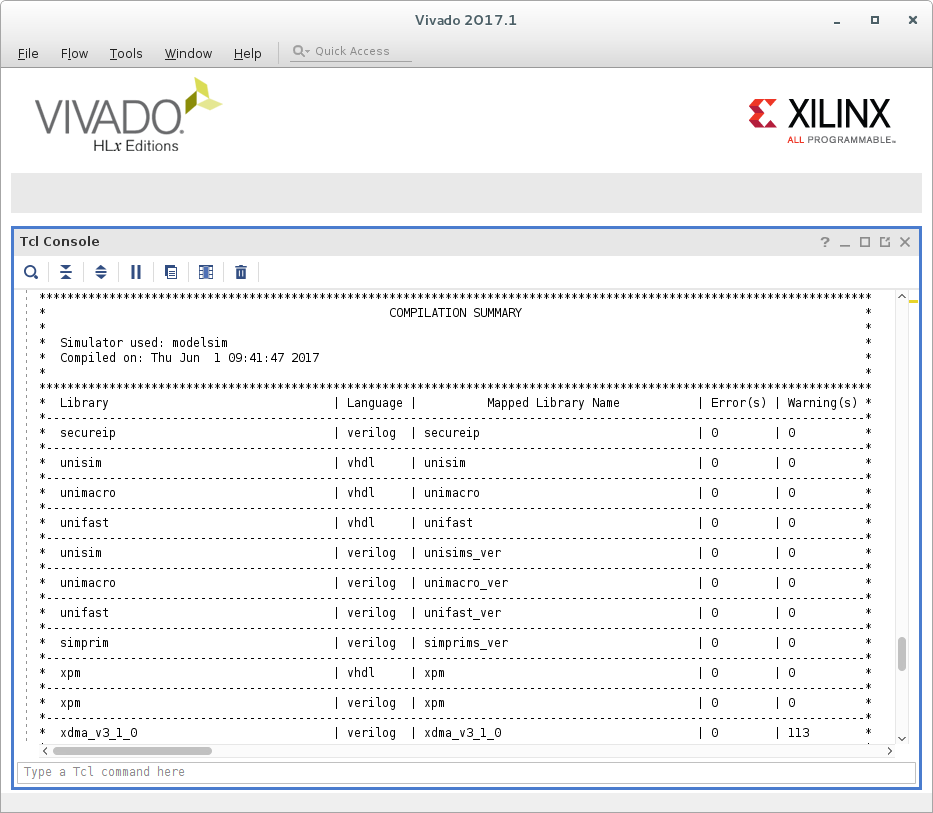
\includegraphics[scale=0.5]{xilinx_vivado_2017_compsimlib_out}
		\captionof{figure}{Vivado 2017.1 Compilation Output with Modelsim DE 10.6a}
	\end{figure}
	\begin{figure}[H]
	\centering\captionsetup{type=figure}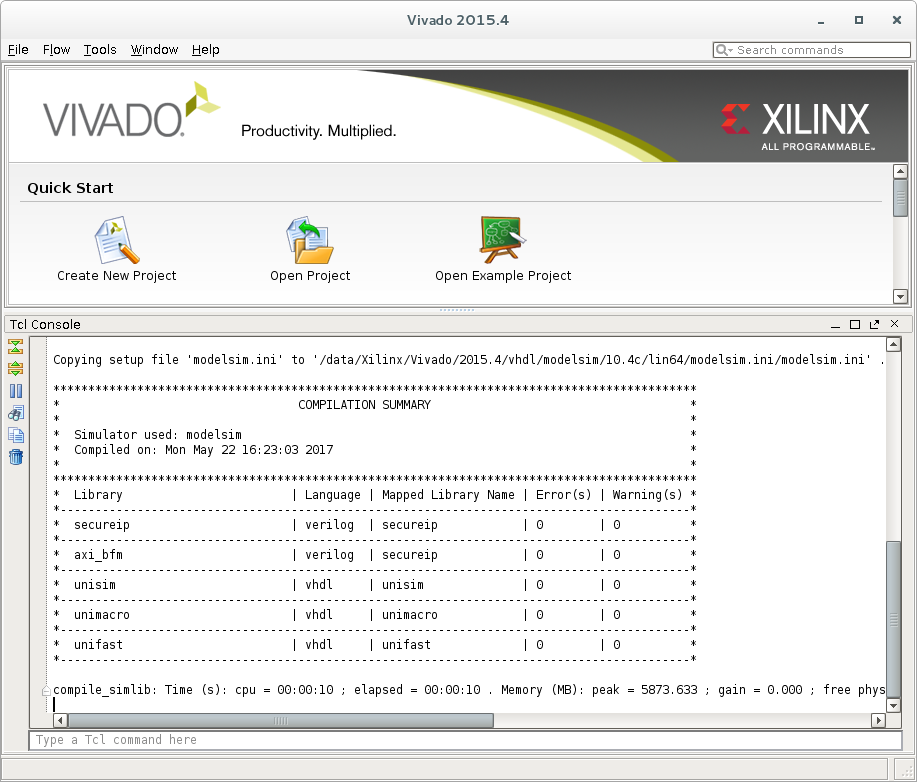
\includegraphics[scale=0.5]{xilinx_vivado_2015_compsimlib_out}
		\captionof{figure}{Vivado 2015.4 Compilation Output with Modelsim DE 10.4c}
	\end{figure}
		\end{enumerate}
\end{flushleft}
\subsection{Compile ISE's simulation libraries}
	This section provides the steps necessary to compile Xilinx ISE's simulation libraries of the Zynq device, for ModelSim.

\begin{flushleft}
	\begin{enumerate}
	 	\item Open a terminal window and switch the user to root:
			\subitem \code{> sudo su -}
		\item Configure the terminal window for Xilinx ISE by sourcing the setup script (for bash):
			\subitem \code{> cd /opt/Xilinx/14.7/ISE\_DS/}
			\subitem \code{> source settings64.sh}
		\item Launch the Xilinx CompXLib GUI:
			\subitem \code{> cd /opt/Xilinx/14.7/ISE\_DS/ISE/bin/lin64}
			\subitem \code{> ./compxlib}

	\begin{figure}[H]
	\centering\captionsetup{type=figure}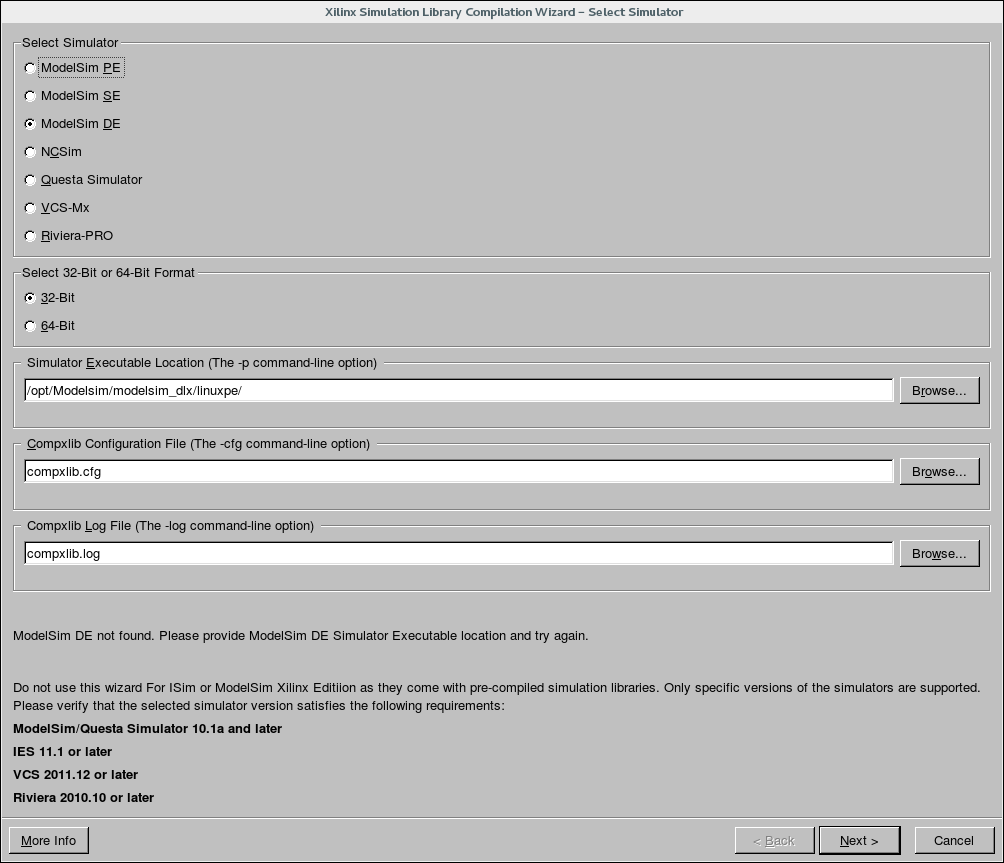
\includegraphics[scale=0.5]{Xilinx_CompXLib_1_Select32bit}
		\captionof{figure}{Compilation Wizard - Select Simulator}
		\label{fig:wizard_page_1}
	\end{figure}

		\item Select ModelSim DE.
		\item Set Simulator Executable Location.
		\item Click ``Next".

	\begin{figure}[H]
	\centering\captionsetup{type=figure}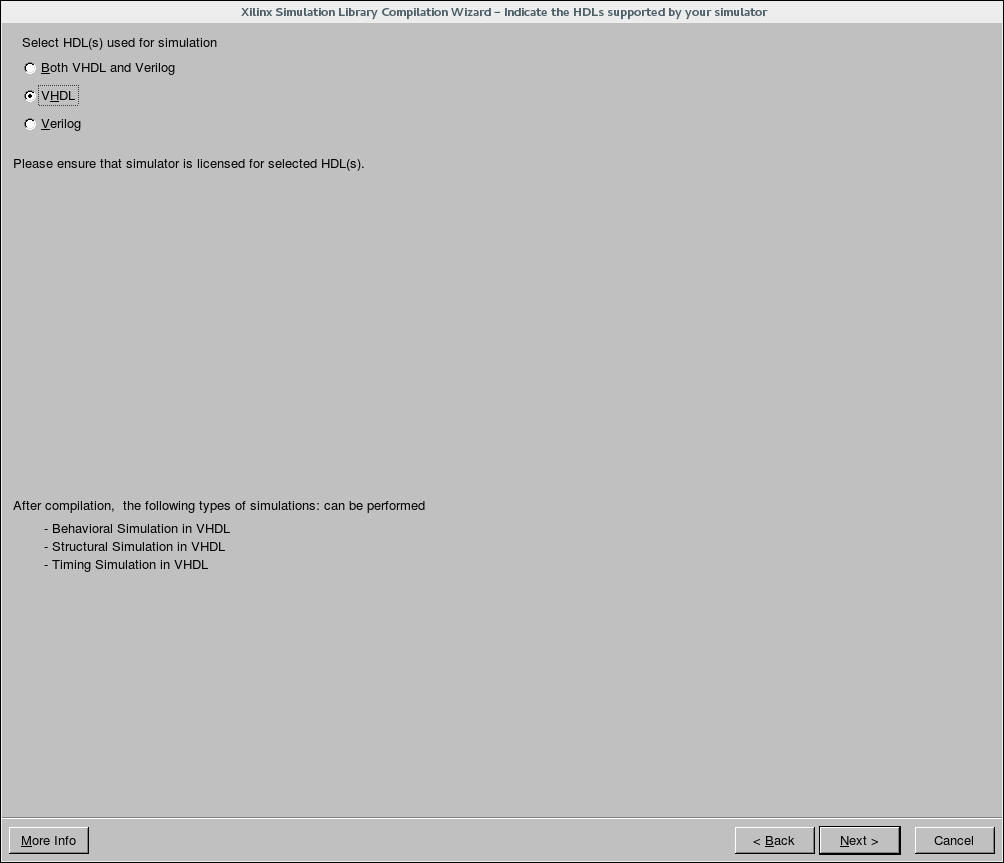
\includegraphics[scale=0.5]{Xilinx_CompXLib_3_VHDLonly}
		\captionof{figure}{Compilation Wizard - HDLs to support simulator}
		\label{fig:wizard_page_3}
	\end{figure}

		\item Select ``VHDL".
		\item Click ``Next".

	\begin{figure}[H]
	\centering\captionsetup{type=figure}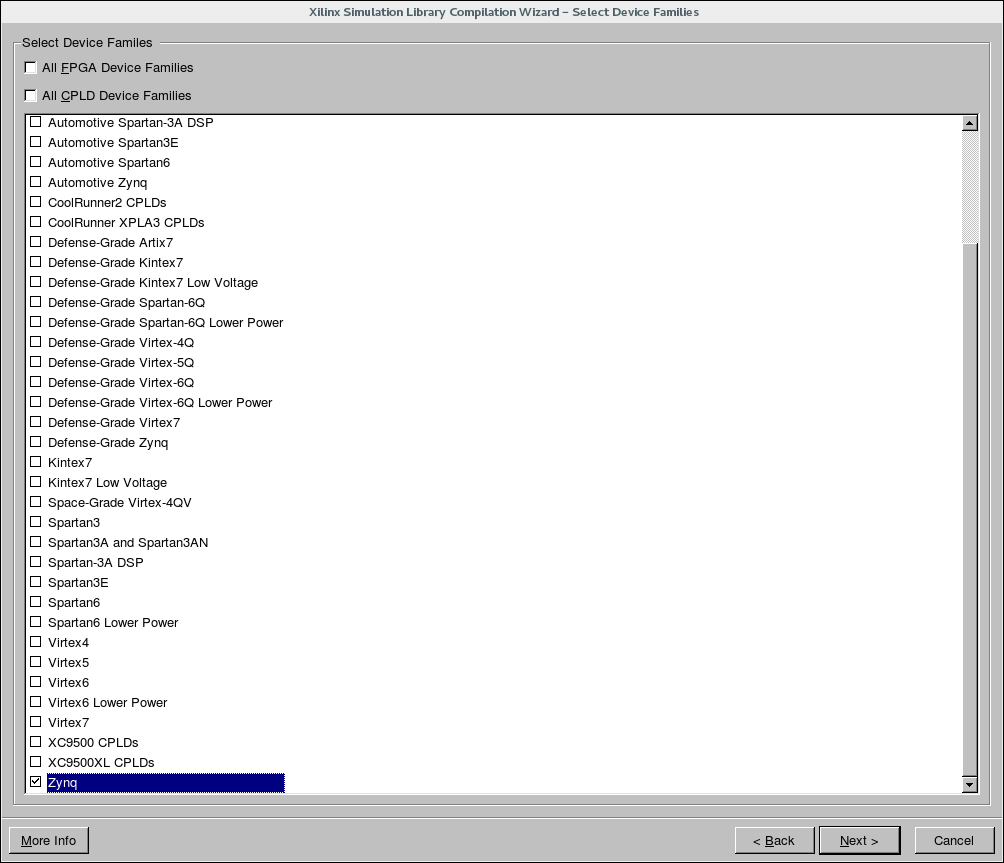
\includegraphics[scale=0.5]{Xilinx_CompXLib_2_SelectZynq}
		\captionof{figure}{Compilation Wizard - Select Device Families}
		\label{fig:wizard_page_2}
	\end{figure}

		\item Uncheck ``All FPGA Device Families".
		\item Uncheck ``All CPLD Device Families".
		\item Check ``Zynq".
		\item Click ``Next".

	\begin{figure}[H]
	\centering\captionsetup{type=figure}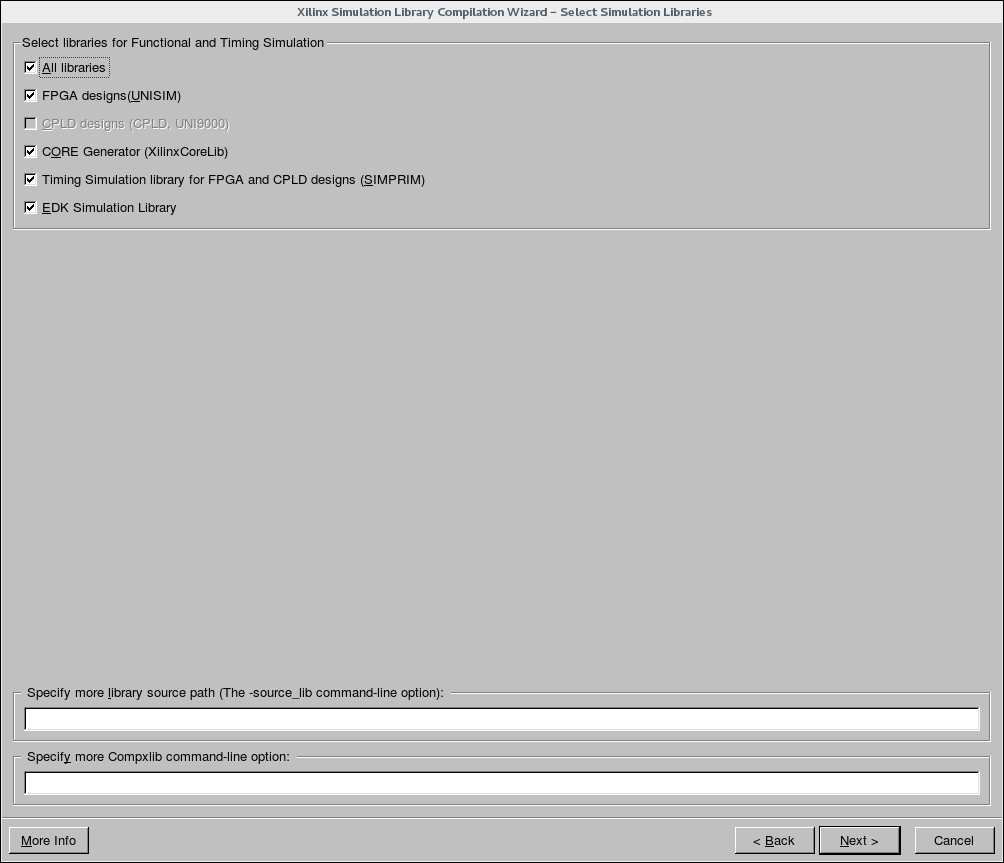
\includegraphics[scale=0.5]{Xilinx_CompXLib_4_BuildAll}
		\captionof{figure}{Compilation Wizard - Select Simulation Libraries}
		\label{fig:wizard_page_4}
	\end{figure}

		\item No change.
		\item Click ``Next".

	\begin{figure}[H]
	\centering\captionsetup{type=figure}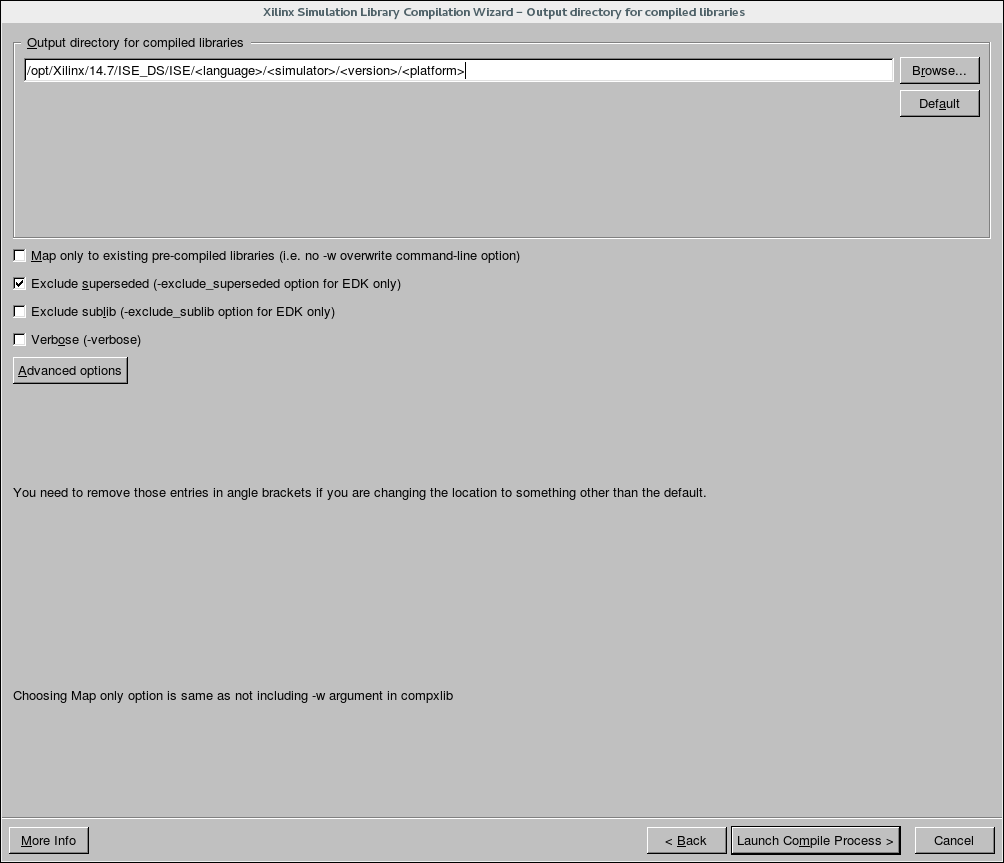
\includegraphics[scale=0.5]{Xilinx_CompXLib_5_SelectDefaults}
		\captionof{figure}{Compilation Wizard - Select Output directory}
		\label{fig:wizard_page_5}
	\end{figure}

		\item Select defaults.
		\item Click ``Launch Compile Process".
			\subitem Note: This step will take approximately 20 mins.

	\begin{figure}[H]
	\centering\captionsetup{type=figure}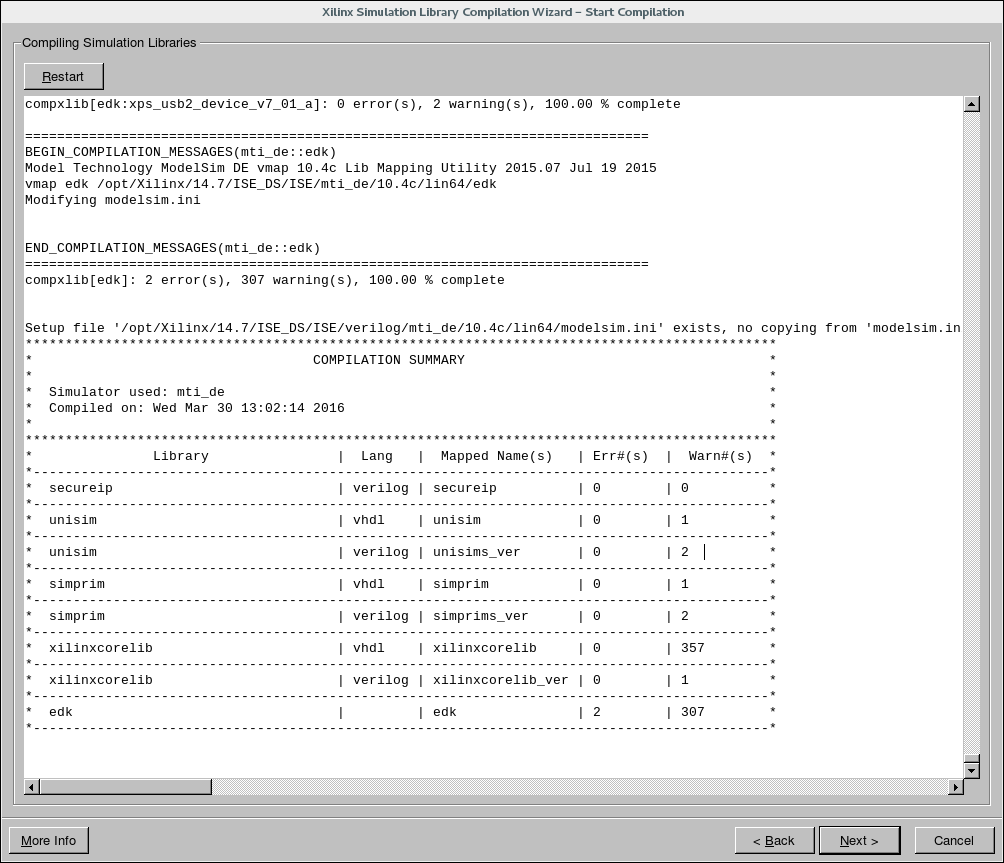
\includegraphics[scale=0.5]{Xilinx_CompXLib_6_CompilationLog}
		\captionof{figure}{Compilation Wizard - Start Compilation}
		\label{fig:wizard_page_6}
	\end{figure}

		\item Click ``Next".

	\begin{figure}[H]
	\centering\captionsetup{type=figure}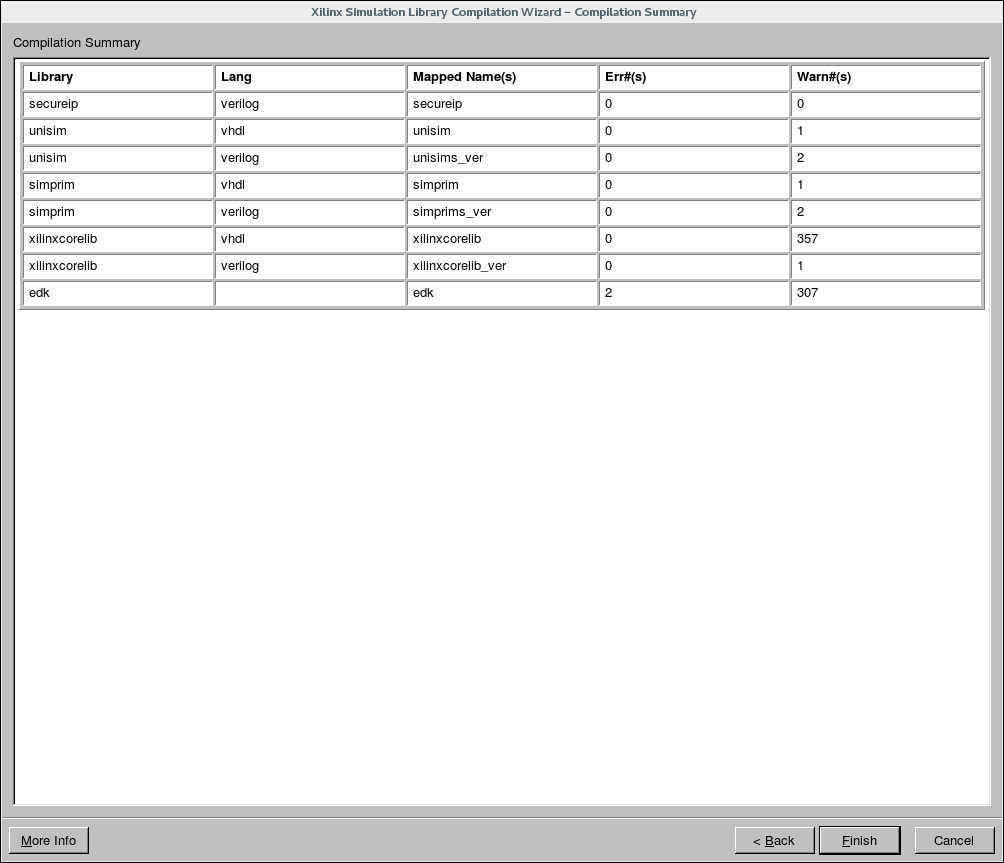
\includegraphics[scale=0.5]{Xilinx_CompXLib_7_CompilationSummary}
		\captionof{figure}{Compilation Wizard - Compilation Summary}
		\label{fig:wizard_page_7}
	\end{figure}


		\item Click ``Finish".
	\end{enumerate}

\newpage

\end{flushleft}

\section{Modify ``modelsim.ini'' to include path to built library}
	This section details the steps to modify the ``\texttt{modelsim.ini}'' file.

	\begin{enumerate}
		\item Browse to the install directory of ModelSim
			\subitem \code{> cd /opt/Modelsim/modelsim\_dlx}
		\item Open the modelsim.ini file as the root user
			\subitem \code{> vi modelsim.ini}
		\item Locate the bottom of the ``\texttt{[Library]}" section and add the following for Vivado:
			\subitem unifast = /opt/Xilinx/Vivado/2017.1/vhdl/modelsim/10.6a/lin64/unifast
			\subitem unisim = /opt/Xilinx/Vivado/2017.1/vhdl/modelsim/10.6a/lin64/unisim
		\item Or, add the following for ISE:
			\subitem xilinxcorelib = /opt/Xilinx/14.7/ISE\_DS/ISE/vhdl/mti\_de/10.4c/lin64/xilinxcorelib
			\subitem unisim = /opt/Xilinx/14.7/ISE\_DS/ISE/vhdl/mti\_de/10.4c/lin64/unisim

	\end{enumerate}
\iffalse
\newpage
\begin{appendices}
\appendix
\section{Appendix - Acronym/Definitions} \label{App:AppendixA}
\begin{flushleft}
\end{flushleft}
\newpage

\end{appendices}
\fi
\end{document}
